%! TEX root = ../main.tex
\documentclass[../main.tex]{subfiles}
\begin{document}
\section{Verfahren}
\subsection{Selective Laser Melting}
Im Jahr 1995 wurde nun ein dem SLA ähnliches Verfahren entwickelt, das Selective-Laser-Melting-Verfahren. Bei diesem wird statt dem Üblichen Photosensitiven UV-Kunstharz und einem UV-LCD feinstes Metallgranulat mit einem herkömmlichen Laser verwendet, welcher dieses in einem Pulverbett geanau zusammenschweißt. \parencite{3FAKTUR_1}
\begin{figure}[h]
\begin{center}
	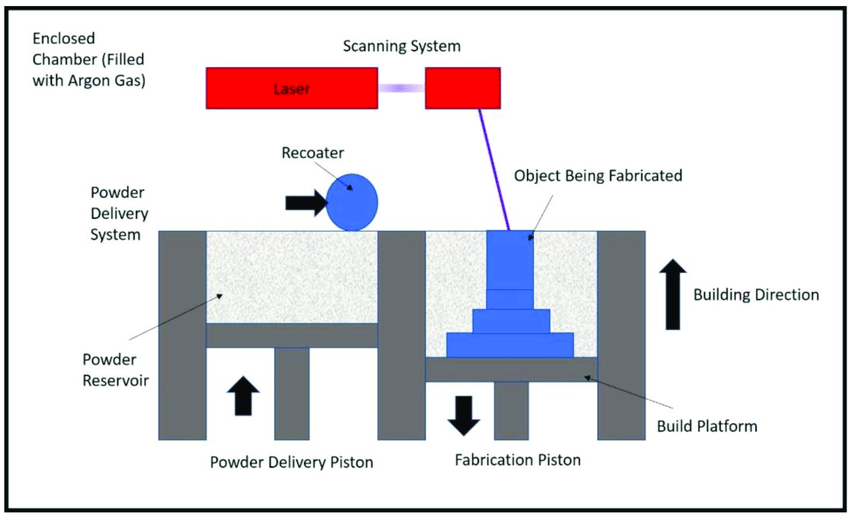
\includegraphics[width=.5\textwidth]{slm_diagram}
	\label{img:slm_diagram}
	\ccaption{Schematischer Aufbau einer SLM-Maschine}{\url{https://www.researchgate.net/publication/326891428/figure/fig1/AS:659597278855194@1534271654724/Schematic-diagram-of-the-selective-laser-melting-SLM-process.png}}
\end{center}
\end{figure}	
SLM ist ein Schichten-basierendes Verfahren. Das bedeutet, es trägt Schicht für Schicht auf
einer Bauplatform auf, welche sich danach nach unten bewegt um eine neue Schicht aufzutragen. 
Hinzu kommt, dass SLM ein Pulverbett-Verfahren ist, was wiederrum bedeutet das eine neue perfekt ebene Schicht auf dem Baustück aufgetragen werden muss nach jedem Absenken der Platform.
Hierfür ist ein Wiederbeschichtungsroller vorhanden. Nach jeder Absenkung des Druckbettes wird über die Pulverlieferungsplatte die exakt gleiche Menge an Granulat nachgeliefert, welche dann vom Wiederbeschichtungsroller eben verteilt wird am Druckbett. 

Der grundlegende Aufbau erscheint simpel, jedoch ist die Umsetzung um einiges komplexer.
Zum einen muss der Laser optimal eingestellt sein für jedes Material, da ansonsten zu viel oder wenig geschmolzen wird.
Auch zu bedenken ist die Reinigung die nach jedem Druck stattfinden muss, wie z.B. die Filterung des Pulvers um falsch verschmolzene Teile auszufiltern, da diese beim nächsten Druck den Roller beschädigen und den Druck verformen könnten. Dabei muss beachtet werden, dass das Pulver dennoch nicht ewig hält und nach einer gewissen Menge an Durchläufen ersetzt werden muss, da ansonsten $D_{10}$ \& $D_{90}$ und der Anteil an $D_{90}$-Teilchen im PSD (PSD, Particle Size Distribution) stark ansteigen, wie in \cite{YI2021524} dargestellt wird anhand von In718-Pulver. 
Außerdem lässt sich im SLM-Verfahren auch über das Offset des Wiederbeschichtungsrollers zum Bett die Schichtdicke bestimmen, was die Produktionszeit stark senken kann.

Dennoch ist die Vielseitigkeit der Grund warum SLM sich so großer Beliebtheit erfreut. Mit verschiendenen Temperaturen des Lasers lassen sich viele Materialien verarbeiten, die Schichtdicke bestimmt auch direkt die Druckdauer, da dickere Schichten zu weniger benötigten Schichten führen, was die Menge an Zeit die durch den Roller verbraucht wird verringert.

Eine solche Veränderung führt aber zu Detailverlust und damit hergehend gröberen Teilen, welche nachbearbeitet werden müssen (Polierung, Schleifung, Drehen, etc.). 
\end{document}
